\documentclass[5p,twocolumn]{elsarticle}
\usepackage{amsmath}
\usepackage{hyperref} % added [draft] to avoid compilation issues that happen if a link is split and appears in two pages
%\modulolinenumbers[5]
\addtolength{\textheight}{8mm}
\addtolength{\textwidth}{4mm}
\addtolength{\voffset}{-10mm}
\addtolength{\hoffset}{-3mm}

\bibliographystyle{elsarticle-num-names}


% ACM template
%
%\documentclass[acmtog,anonymous,timestamp,review]{acmart}
%
%\usepackage{booktabs} % For formal tables
%




% My TK added packages and commands

	\newif\ifcolorrevise
	
	\colorrevisetrue

	% for for using hyperref and elsarticle-num-names together in order to get \citeauthor to work
	\makeatletter
	\providecommand{\doi}[1]{%
	  \begingroup
	    \let\bibinfo\@secondoftwo
	    \urlstyle{rm}%
	    \href{http://dx.doi.org/#1}{%
	      doi:\discretionary{}{}{}%
	      \nolinkurl{#1}%
	    }%
	  \endgroup
	}
	\makeatother

	% have multiline subfigure captions be centered
	\usepackage[labelformat=parens]{subcaption} % subfigures
	\captionsetup[subfigure]{justification=centering}
	\captionsetup{subrefformat=parens} % pure refernce subfigure with parentheses: fig.10a and (b)
	%\renewcommand\thesubfigure{(\alph{subfigure})} % refernce subfigure always with parentheses: fig.10(a) and (b)

	\captionsetup[figure]{labelfont={bf},name={Fig.},labelsep=period} % use `Fig.' for figure subscript instead of `Figure'
	
	\usepackage[export]{adjustbox} % [right] alignment for includegraphics
	
	\usepackage{rotating} % turn env for rotating text in figures

	\usepackage{wrapfig} % inline figures

	% tables
	\usepackage{multirow} % multicolumn, multirow
	\usepackage{colortbl} % \cellcolor{<color>}
	\newcolumntype{C}[1]{>{\centering\arraybackslash}m{#1}}   %% centered
	\newcolumntype{R}[1]{>{\raggedleft\arraybackslash}m{#1}}  %% right aligned

	\usepackage[capitalise]{cleveref} % automatically add `Fig.'  etc before a reference.

        \usepackage{ amssymb } % \therefore
	
	\newcommand{\degree}{^\circ}
	
	\usepackage[binary-units]{siunitx} % mm and stuff
	\sisetup{per-mode = symbol}
	\DeclareSIUnit\pixel{px}

	\usepackage{units} % \nicefrac{3}{8}
	
	
	
	\DeclareMathOperator*{\argmax}{arg\,max}
	\DeclareMathOperator*{\argmin}{arg\,min}
	
	\DeclareMathOperator{\abs}{abs} % absolute function

	\usepackage{amsthm} % \begin{proof}
	\newtheorem{lemma}{Lemma}[section]
	\theoremstyle{definition}
	\newtheorem{definition}{Definition}[section]

	\usepackage[inline]{enumitem} % inline enumerate*

	\usepackage[toc,page]{appendix} % appendicces
	
	\usepackage{pgfplots}
	\usepackage{pgfplotstable} % tikzpicture table plots
	\pgfplotsset{compat=1.15}
	\usetikzlibrary{backgrounds}

	\usepackage[noend]{algpseudocode} % algorithmic
	\usepackage{algorithm} % wrapper for pseudocode to give a caption and label

	\newcommand{\pluseq}{\mathrel{+}=} %pluseq symbol
	\usepackage{upgreek} % \uplambda

	\usepackage{listings} % for listing C++ code instead of pseudocode
	\lstset{ 
      breaklines=true,                 % sets automatic line breaking
      basicstyle=\ttfamily,
      mathescape
    }




    % \usepackage[disable]{todonotes} % notes not showed  
    % \usepackage[draft]{todonotes}   % notes showed
    \usepackage{color,soul} % caps, highlight (\hl)

	\newcommand{\comment}[1]{}
	
    \newcommand{\todo}[1]{\hl{#1}}
    
	\newcommand{\temp}[1]{\textcolor[rgb]{0, 0, 0.2}{#1}}
	\newcommand{\tim}[1]{\temp{\todo{[Tim: #1]}}}
	\newcommand{\jun}[1]{\temp{\todo{[Jun: #1]}}}
	
	\newcommand{\old}[1]{\textcolor{gray}{#1}}
	\usepackage[normalem]{ulem}
	\newcommand{\stkout}[1]{\ifmmode\text{\sout{\ensuremath{#1}}}\else\sout{#1}\fi}
	
	% Revise macro (usage: \revise{old}{new})
	\newcommand{\revise}[2]{#2}
	% Version a) First arg red and striked out, second argument green
	%\newcommand{\revise}[2]{\textcolor{red}{\stkout{#1}}\textcolor{blue}{#2}}
	%\newcommand{\revise}[2]{{\color{red}{#1}\color{blue}{#2}}}
	% Version b) First arg ignored, second argument green
	\ifcolorrevise
	\renewcommand{\revise}[2]{{\color{blue}{#2}}}
	\fi
	% Version c) First arg ignored, second argument unchanged (for final draft)
	%\newcommand{\revise}[2]{#2}
	%\newcommand{\revise}[2]{#1}

	\newcommand{\outdated}[1]{{\color{red}{#1}}}

	\setulcolor{red}

	\usepackage[normalem]{ulem} % squigly underline

	\renewcommand\floatpagefraction{.8}


	\newlength{\figwidth}
	\newlength{\figwidthTwo}
	\newlength{\figwidthTree}
	\newlength{\figheight}
	\newlength{\figheightTwo}
	\newlength{\tempheight}
	\newlength{\tempheightTwo}

	% deal with missing images which are not directly included in the repo
	\iftrue
	\newcommand{\noimage}[1]{%
	  \setlength{\fboxsep}{-\fboxrule}%
	  \fbox{\phantom{\rule{10pt}{10pt}} Missing file: \path{#1} \phantom{\rule{10pt}{10pt}}}% Framed box
	}
	\let\includegraphicsoriginal\includegraphics
	\renewcommand{\includegraphics}[2][width=\textwidth]{\IfFileExists{#2}{\includegraphicsoriginal[#1]{#2}}{\noimage{#2}}}

	\fi
% ENd of TK's added packages and commands



\begin{document}
\baselineskip11pt 

\begin{frontmatter} 

\title{Mechanical interlocking microstructure to enhance adhesion between chemically incompatible plastics}

%\author{Paper ID: xxx}

\author[um]{Tim Kuipers}
\author[tud]{Nadine Duursma}
%\cortext[cor1]{Corresponding author}
%\author[cuhk]{Charlie C. L. Wang}
% \ead{cwang@mae.cuhk.edu.hk}
\address[um]{employee number 909290}
\address[tud]{student number 4665236}



\begin{abstract}
Using incompatible materials in FDM 3D printing is difficult because the materials do not adhere to each other.
In order to bond two shapes of incompatible materials together as good as possible, we investigate 
mechanically interlocking structures.
\end{abstract}

%
% The code below should be generated by the tool at
% http://dl.acm.org/ccs.cfm
% Please copy and paste the code instead of the example below.
%
%\begin{CCSXML}
%\end{CCSXML}

%\ccsdesc[500]{Computer systems organization~Embedded systems}
%\ccsdesc[300]{Computer systems organization~Redundancy}
%\ccsdesc{Computer systems organization~Robotics}
%\ccsdesc[100]{Networks~Network reliability}

%\begin{keyword} 
%keywords
%\end{keyword}

\end{frontmatter}




%  \temp{%Table of contents just for reviewing purposes
%  \tableofcontents
%  }

\section{Introduction}
Our project is centered around the PhD research of Tim Kuipers, so you might want to expect that together we may shift more work than other group projects.

\medskip

If one wishes to print one part consisting of two incompatible materials then some interlocking geometry will need to be introduced at the interface between these two materials in order to make these two materials adhere to each other mechanically.
We consider two materials, a hard one (shown in green) and a soft one (in cyan), which are placed next to each other such that the interface is horizontal
and we will consider a tensile for is applied orthogonal to the interface.

The structure consists of parallel beams of alternating materials in some layers, and in other layers the beams of both materials are rotated, so that they connect the various beams of the former, thusly interlocking the materials.
We want to optimize the structure such that it can withstand the highest tensile force, for an arbitrarily large interface;
that is, we want to optimize the effective ultimate tensile strength of the interlocking micro-structure.
We want to optimize our structure such that none of the components of breaks or yields at the highest applied force.
On the other hand we would like our structure to be as small as possible, which is captured in both constraints and objective functions.

We consider two closely related interlocking geometries consisting of beams of either material connected 
Both of these geometries are limited by manufacturing constraints:
\begin{itemize}
	\item heights are a discrete multiple of the layer thickness $h_\text{min}$
	\item widths are continuous, but at least twice the nozzle size $w_\text{min}$
	\item the width of a very long beam may be smaller: at least once the nozzle size $w_\text{min}$
\end{itemize}


We consider two orientations of the interlocking pattern:
\begin{description}
	\item[Straight] even beams (`cross beams') are aligned parallel to the interface and odd beams (`fingers') are perpendicular
	\item[Diagonal] even beams and odd beams (both `fingers') are at equal and opposite angles w.r.t. the interface.
\end{description}

\begin{figure}[H]
	\centering
	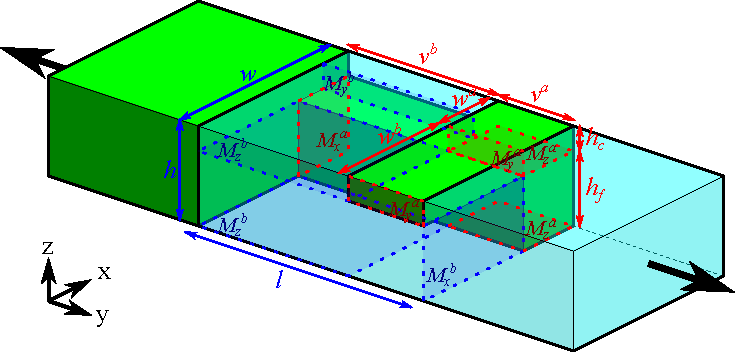
\includegraphics[width=\columnwidth]{sources/method/straight_model_v3.pdf}
	\caption{
		One straight unit cell connecting material $a$ (left) to material $b$ (right).
		Failure can happen along the fingers ($M_x$), along the cross beams ($M_y$) or at the interface between the two ($M_z$) for either material.}
	\label{fig:failure_modes}
\end{figure}

\begin{figure}[H]
	\centering
	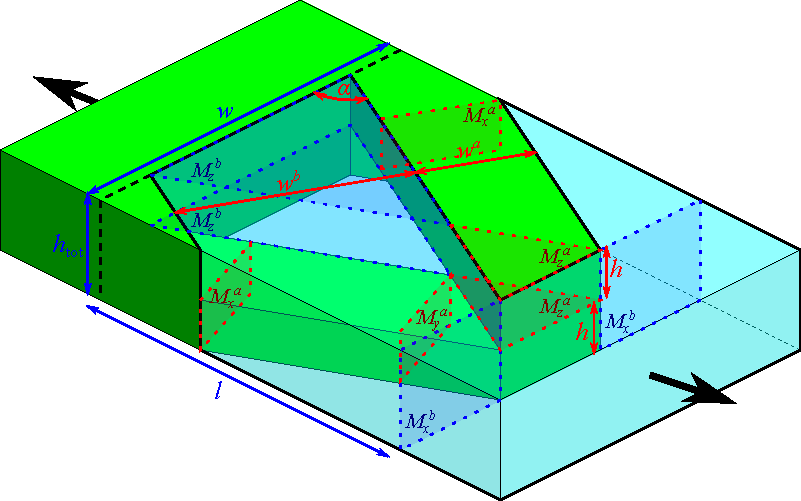
\includegraphics[width=\columnwidth]{sources/method/diagonal_model_v3.pdf}
	\caption{
		One diagonal unit cell connecting material $a$ (left) to material $b$ (right).
		Failure can happen along both the fingers ($M_x$), twice along one finger ($M_y$) or at the interface between the two fingers ($M_z$) for either material.}
	\label{fig:diagonal_model}
\end{figure}



\section{Straight Orientation}





\Cref{fig:failure_modes} shows one cell of the straight structure, along with the design variables and the failure modes.
The optimization then consists of the following:

\begin{align}
	& \max \frac{F}{\left( w^a + w^b \right) \left( h_\text{f} + h_\text{c} \right) } \\
	& \min h_\text{f} h_\text{c} \\
	\text{subject to} & \nonumber \\
	w^m &\ge w_\text{min}^m \\
	v^m &\ge v_\text{min}^m \\
	h_\text{f} &\ge h_\text{min} \\
	h_\text{c} &\ge h_\text{min} \\
	v^a + v^b &\le v_\text{max} \\
	\frac{ F }{ w^m h_\text{f} } &\le \sigma^m_\text{yield} &&\text{ Tension failure } M_x^m \\
	\frac{ 3 F }{ 4 v^m h_\text{c}} &\le \tau^m 			&&\text{ Shear failure } M_y^m \\
	\frac{ 3 F }{ 4 v^m w^m } &\le \tau^m_\text{Z} 			&&\text{ Shear failure } M_z^m \\
	\frac{ 3 F w^b }{ 4 \left( v^a \right)^2 h_\text{c} } &\le \sigma^a_\text{yield}			&&\text{ Bending failure } M_y^a \\
	\frac{ 3 F w^a }{ 4 \left( v^b \right)^2 h_\text{c} } &\le \sigma^b_\text{yield}			&&\text{ Bending failure } M_y^b \\
	& \text{for both materials } && m \in \{a, b\} \nonumber
\end{align}

\iffalse

\paragraph{Monotonicity Analysis}
\begin{align*}
	\min & 1 - \frac{F}{\left( w^a + w^b \right) \left( h_\text{f} + h_\text{c} \right) }
																		&& F^-, w^{a+}, w^{b+},  h_\text{f}^+, h_\text{c}^+\\
	\text{subject to} & \nonumber \\
	1 - \frac{w^m }{w_\text{min}^m} &\le 0    							&& w^{m-} \\
	1 - \frac{v^m }{w_\text{min}^m} &\le 0    							&& v^{m-} \\
	1 - \frac{h_\text{f}}{h_\text{min}} &\le 0 							&& h_\text{f}^- \\
	1 - \frac{h_\text{c}}{h_\text{min}} &\le 0 							&& h_\text{c}^- \\
	\frac{v^a + v^b}{ v_\text{max} }  - 1&\le 0 						&& v^{a+}, v^{b+} \\
	\frac{ F }{ w^m h_\text{f} \sigma^m_\text{yield} } - 1&\le 0 		&& F^+, w^{m-}, h_\text{f}^- \\
	\frac{ 2 F }{ 3 v^m h_\text{c} \tau^m } - 1 &\le 0 					&& F^+, v^{m-}, h_\text{c}^- \\
	\frac{ 2 F }{ 3 v^m w^m \tau^m_\text{Z} } - 1 &\le 0 					&& F^+, v^{m-}, w^{m-} \\
	\nonumber \\
	F^m &= \sigma^m w^m h_\text{f} \\
	\dots \\
	& \text{for both materials } m \in \{a, b\}
\end{align*}
\fi


This looks like a multi-objective optimization problem, but without the second objective the problem is under-constrained.
Adding the second objective actually means there's one unique solution - rather counter-intuitively.

The $v^m$ variables don't figure in the objective, but they do appear in the constraints and therefore are also subject to the optimization.

We should be able to find analytical solution(s), depending on the size of $v_\text{max}$ w.r.t. the other constraints.

Possible extensions:
\begin{itemize}
	\item Consider multiple repetitions of the cell in the loading direction.
	\item Consider tensile load in Z direction.
	\item Consider FEM model.
\end{itemize}

\iffalse
Formula is given by this? :
% from https://skyciv.com/docs/tutorials/beam-tutorials/bending-moment-equations/
\begin{align*}
	\sigma_\text{bend} &= \frac{M r}{I} \\
	&= \frac{M \nicefrac12 v}{I} \\
	M_\text{max} &= \frac{v L}{12} \text{ for distributed force and fixed sides} 
\end{align*}
\fi













\section{Slanted design}

Another option is to place the fingers under an angle as shown in \autoref{fig:diagonal_model}.
There are four design variables: the finger width of both materials: $w^a$ and $w^b$, the finger rotation angle $\alpha$, and the layer thickness $h$.




The goal is to maximize the strength, while accounting for the failure modes in the constraints.
With that, the optimization problem can be formulated as follows:

\begin{align}
	& \max \frac{F \sin \alpha}{\left( w^a + w^b \right) 2h } \\
	\text{subject to:} & \nonumber \\
	w^m &\ge w_\text{min}^m \\
	h &\ge h_\text{min} \\
	\alpha_{min} &\le \alpha \le \alpha_{max}\\
	w^a + w^b &\le w_\text{max} \\
	\frac{ F \sin \alpha}{ w^m h } &\le \sigma^m_\text{yield} &&\text{ Tension failure } M_x^m \\
	\frac{ 3 F \cos \alpha }{ 4 w^m h_\text{c}} &\le \tau^m 			&&\text{ Shear failure } M_x^m \\
	\frac{ 3 F \sin \alpha \cos \alpha }{ \left(w^m \right)^2 } &\le \tau^m_\text{Z} 			&&\text{ Shear failure } M_z^m \\
	\frac{ 3 F w^b }{ 8 \sin \alpha \left(w^a \right)^2 h} & \le \sigma^a_\text{yield}			&&\text{ Bending failure } M_x^a \\
	\frac{ 3 F w^a }{ 8 \sin \alpha \left(w^b \right)^2 h} & \le \sigma^b_\text{yield}			&&\text{ Bending failure } M_x^b \\
	& \text{for both materials } && m \in \{a, b\} \nonumber
\end{align}




%\section*{References}
\interlinepenalty=100000 % prevents pdfendlink ended up accross pages error. see https://tex.stackexchange.com/a/449633/129190
\bibliography{99_mybib}


%\begin{appendices}
%\input{19_edge_discretization}
%\end{appendices}

\end{document}
